\documentclass{article}


\usepackage{arxiv}
\usepackage{algorithm,algpseudocode}

\usepackage[utf8]{inputenc} % allow utf-8 input
\usepackage[T1]{fontenc}    % use 8-bit T1 fonts
\usepackage{hyperref}       % hyperlinks
\usepackage{url}            % simple URL typesetting
\usepackage{booktabs}       % professional-quality tables
\usepackage{amsfonts}       % blackboard math symbols
\usepackage{nicefrac}       % compact symbols for 1/2, etc.
\usepackage{microtype}      % microtypography
\usepackage{lipsum}
\usepackage{amsmath}
\usepackage{amssymb}
\usepackage{textcomp}
\usepackage[dvipsnames]{xcolor}
\usepackage{graphicx}
\usepackage{subcaption}
\usepackage{bbold}
\usepackage{bm}
\newcommand{\CO}{\mathcal{O}}
\usepackage{wrapfig}
\newcommand\subfig[2]{{Fig.~\ref{#1}{#2}}}
\newcommand\fig[1]{{Fig.~\ref{#1}}}
\usepackage[super]{nth}
\usepackage{dirtytalk}
\usepackage{braket}
%\usepackage{blindtext}
%\usepackage{tcolorbox}
%\usepackage{graphicx}

\usepackage{empheq}
\usepackage[most]{tcolorbox}
\tcbset{highlight math style={boxsep=1mm,colback=blue!30!red!10!white}}

\title{Préparation de Mac pour le TP}


\author{
Pour toute question, veuillez contacter\\
 Juliane U. Klamser\\%\thanks{website}\\
  Gulliver,  ESPCI\\
  Paris \\
  \texttt{Juliane.Klamser@espci.psl.eu} \\
}

\begin{document}
\maketitle

\tableofcontents

%\begin{abstract}
%Bla bla
%\end{abstract}


% keywords can be removed
%\keywords{First keyword \and Second keyword \and More}

\section{Installer les outils de la ligne de commande}
\subsection{La solution la plus simple: Installation Xcode}
Si vous installez Xcode, vous pouvez utiliser Xcode comme éditeur de code. Vous n'avez pas besoin d'installer d'autres logiciels pour éditer les codes.
Allez sur l'App Store et cherchez Xcode. Téléchargez et installez cette application.
\begin{figure}[H]
\center
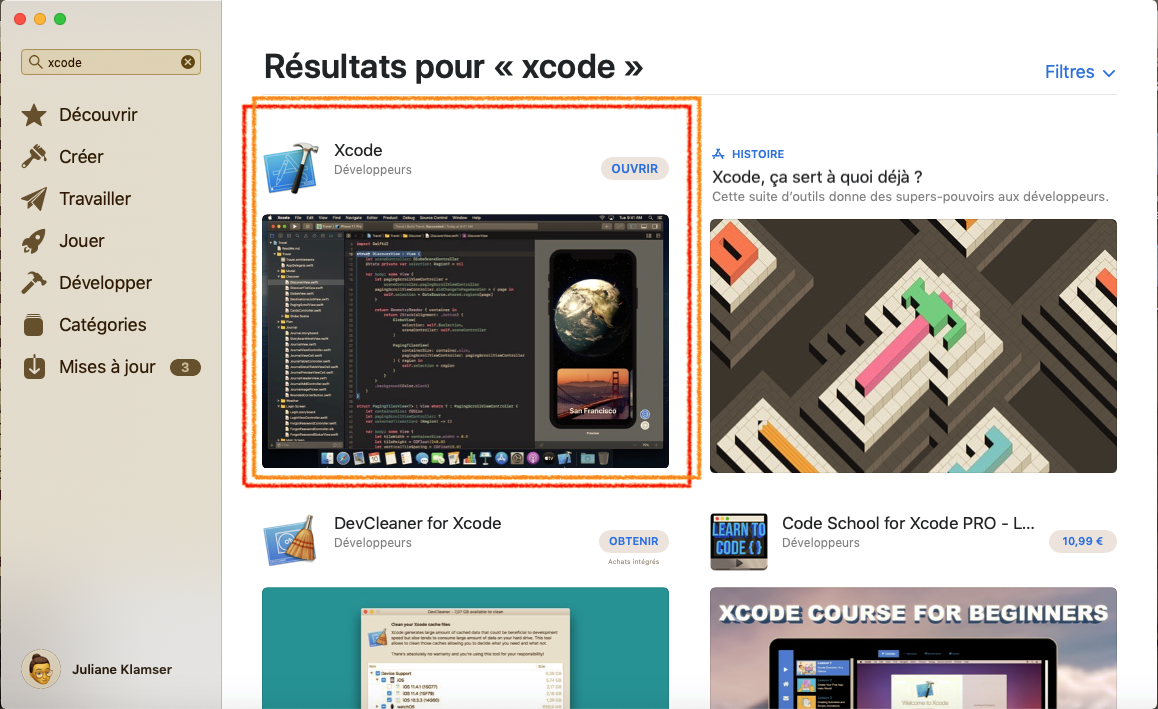
\includegraphics[width=0.75\textwidth]{Plots/AppStoreXcode.png}
%\caption{Choisissez la version qui est compatible avec votre ordinateur.}
\end{figure}
\subsection{Installation sans Xcode}
Il est possible que vous ne soyez pas en mesure d'installer Xcode ou que vous ne souhaitiez pas l'installer.  Dans le premier cas, vous pouvez envisager de \textbf{mettre à jour votre système d'exploitation} (cliquez sur la pomme dans la barre de menu -> à propos de ce Mac -> overview -> mise à jour). Une fois votre système mis à jour, vous n'aurez probablement plus de problèmes pour télécharger Xcode. En outre, cela permet d'éviter d'autres problèmes dans ce qui suit.

Si vous ne pouvez ou ne voulez vraiment pas installer Xcode, procédez comme suit:\\
Vous pouvez installer les outils de la ligne de commande sans Xcode. Pour cela, vous devez lancer l'application appelée Terminal. Cette application se trouve dans /Applications/Utilitaires/. Vous pouvez également la rechercher avec "Spotlight" (cmd + espace ou loupe dans le coin supérieur droit de la barre de menu).
\begin{figure}[H]
\begin{subfigure}[c]{0.5\textwidth}
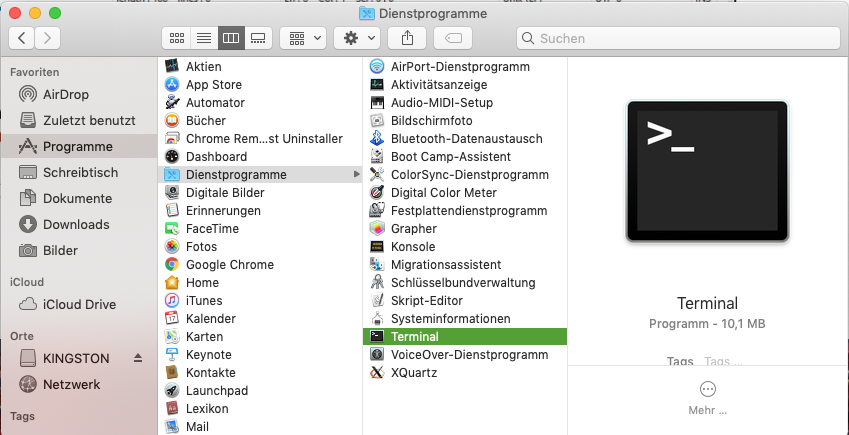
\includegraphics[width=1\textwidth]{Plots/Terminal.png}
\subcaption{Applications/Utilitaires/}
\end{subfigure}
\begin{subfigure}[c]{0.5\textwidth}
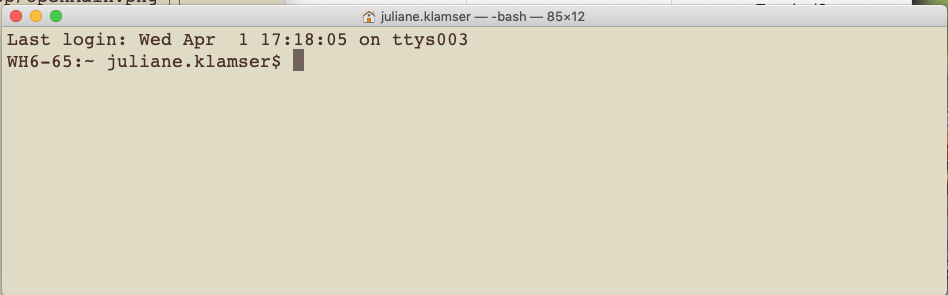
\includegraphics[width=1\textwidth]{Plots/Terminal2.png}
\subcaption{C'est votre terminal, qui pourrait vous sembler un peu différent. Vous pouvez modifier les paramètres de couleur et de police, pour cela, voir \fig{Sub:T3}.}
\end{subfigure}
\center
\begin{subfigure}[c]{0.5\textwidth}
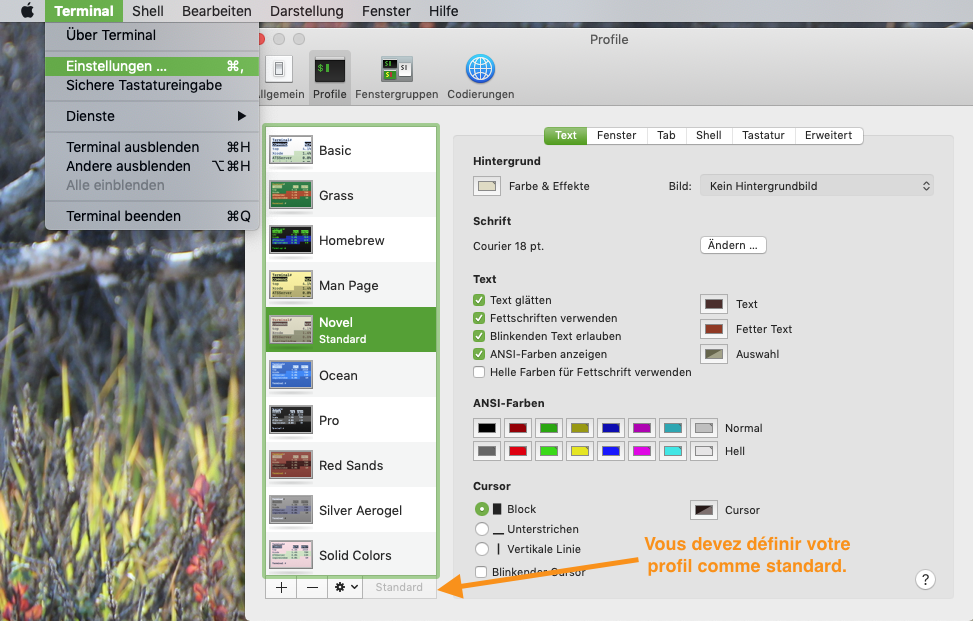
\includegraphics[width=0.8\textwidth]{Plots/Terminal3.png}
\subcaption{Modifiez les paramètres de couleur et de caractères de votre terminal. Barre de menu $\rightarrow$ terminal $\rightarrow$ propriétés $\rightarrow$ profil. Vous devez définir votre profil comme standard. \label{Sub:T3}}
\end{subfigure}
\caption{Le terminal se trouve dans /Applications/Utilitaires/. Vous pouvez également la rechercher avec "Spotlight" (cmd + espace ou loupe dans le coin supérieur droit de la barre de menu). L'image est en allemand ;) \label{F:HowToFindTerminal}}
\end{figure}



Vous devez copier-coller la commande suivante dans le terminal et confirmer la commande avec ENTRÉE.
\begin{tcolorbox}[width=\textwidth,colframe=Bittersweet,colback={black},title={Ceci est le terminal},outer arc=0mm,colupper=white]    
      \large\textbf{xcode-select --install}
\end{tcolorbox}
Il devrait vous sembler comparable à cela :
\begin{figure}[H]
\center
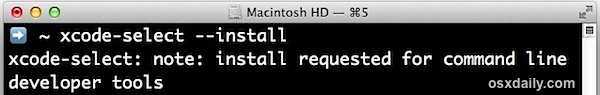
\includegraphics[width=0.75\textwidth]{Plots/install-command-line-tools-os-x.jpg}
\end{figure}

Une fenêtre contextuelle de mise à jour du logiciel apparaîtra et vous posera des questions : "La commande xcode-select nécessite les outils de développement en ligne de commande. Choisissez de confirmer en cliquant sur "Installer", puis d'accepter les conditions d'utilisation (n'hésitez pas à les lire attentivement, nous serons là).
\begin{figure}[H]
\center
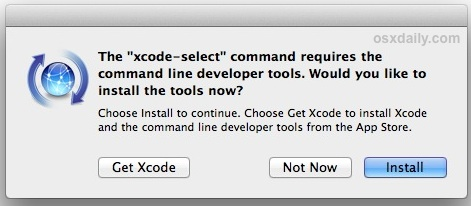
\includegraphics[width=0.6\textwidth]{Plots/confirm-install-command-line-tools-mac-os-x.jpg}
\end{figure}
Attendez que le téléchargement du paquet d'outils en ligne de commande soit terminé, il fera environ 130 Mo et s'installera assez rapidement en fonction de votre vitesse de connexion
\begin{figure}[H]
\center
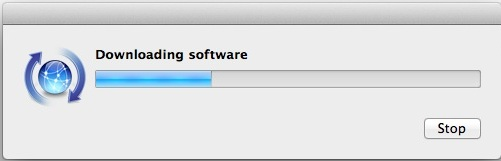
\includegraphics[width=0.6\textwidth]{Plots/downloading-command-line-tools.jpg}
\end{figure}
L'installateur s'en va de lui-même quand il a terminé.

Maintenant, vous avez également besoin d'un éditeur de code.
\subsubsection{éditeur de code\label{S:VisCodAtom}}
Vous pouvez essayer atom \href{https://atom.io}{https://atom.io}\\
ou bien Visual Studio Code \href{https://code.visualstudio.com/download}{https://code.visualstudio.com/download}

Les deux éditeurs de code offrent une option qui vous permettent de travailler simultanément sur le même code avec quelqu'un. C'est très utile pour le projet final, lorsque vous travaillez avec un partenaire sur le même code. Cette fonction est appelée "Teletype" pour atom et "live share" pour Visual Studio Code. 

\section{Installation Xquartz \label{S:InstallXquatz}}
Plus tard, nous aurons besoin de Xquartz, qui permet de faire de la visualisation graphique avec vos codes.
Veuillez télécharger le logiciel ici (utilisez les paramètres par défaut si possible) : \href{https://www.xquartz.org}{https://www.xquartz.org}.
\section{Installation Gnuplot}
Gnuplot est un logiciel qui sert à produire des représentations graphiques en deux ou trois dimensions de fonctions numériques ou de données. Il sera très utile pour tracer des données avec quelques lignes.
\subsection{Installation de homebrew}
Homebrew est un logiciel de gestion de paquets pour macOS gratuit et open-source écrit en ruby. Son but est de simplifier l'installation de programme. Nous l'utiliserons pour installer gnuplot.

Vous devez lancer l'application appelée Terminal (voir \fig{F:HowToFindTerminal}).

Vous devez copier-coller la commande suivante dans le terminal et confirmer la commande avec ENTER.
\begin{tcolorbox}[width=\textwidth,colframe=Bittersweet,colback={black},title={Ceci est le terminal},outer arc=0mm,colupper=white]    
      \large\textbf{ruby -e "\$(curl -fsSL https://raw.githubusercontent.com/Homebrew/install/master/install)" < /dev/null 2> /dev/null}
\end{tcolorbox}
Il vous sera peut-être demandé d'entrer votre mot de passe, veuillez entrer le mot de passe d'utilisateur de votre Mac pour continuer. Lorsque vous tapez le mot de passe, il ne s'affiche pas à l'écran, mais le système l'accepte. Il vous suffit donc de taper votre mot de passe et d'appuyer sur la touche ENTER/RETOUR. Attendez ensuite que la commande se termine.
\subsection{Mise à jour du homebrew}
Nous devons d'abord nous assurer que l'homebrew est à jour.
Vous devez copier-coller la commande suivante dans le terminal et confirmer la commande avec ENTER. Cela peut prendre un certain temps avant de se terminer.
\begin{tcolorbox}[width=\textwidth,colframe=Bittersweet,colback={black},title={Ceci est le terminal},outer arc=0mm,colupper=white]    
      \large\textbf{brew update}
\end{tcolorbox}
Maintenant, copiez-collez la commande suivante dans le terminal, confirmer la commande avec ENTER et attendez que l'installation soit terminée.
\begin{tcolorbox}[width=\textwidth,colframe=Bittersweet,colback={black},title={Ceci est le terminal},outer arc=0mm,colupper=white]    
      \large\textbf{brew upgrade}
\end{tcolorbox}
\subsection{Installation Gnuplot via homebew}
Pour installer des paquets avec home-brew, vous utilisez toujours la syntaxe brew install <nom du paquet>. Pour installer gnuplot, copiez-collez la commande suivante dans le terminal, confirmez avec entrée et attendez la fin de l'installation.
\begin{tcolorbox}[width=\textwidth,colframe=Bittersweet,colback={black},title={Ceci est le terminal},outer arc=0mm,colupper=white]    
      \large\textbf{brew install gnuplot}
\end{tcolorbox}
\subsection{Vérifiez que l'installation est réussie.}
Pour vérifier si l'installation a réussi, copiez-collez la commande suivante dans le terminal, confirmez avec ENTRÉE.
\begin{tcolorbox}[width=\textwidth,colframe=Bittersweet,colback={black},title={Ceci est le terminal},outer arc=0mm,colupper=white]    
      \large\textbf{gnuplot --version}
\end{tcolorbox}
Votre résultat devrait ressembler à ceci (Dans cet exemple, la version de gnuplot est 5.2.)
\begin{figure}[H]
\center
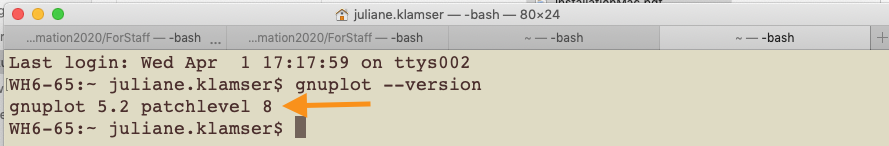
\includegraphics[width=0.6\textwidth]{Plots/GnuplotCheck.png}
\end{figure}
\subsection{Troubleshooting}
Si vous avez un problème pour installer gnuplot via le terminal, veuillez vous rendre sur ce site \href{https://csml-wiki.northwestern.edu/index.php/Binary_versions_of_Gnuplot_for_OS_X}{https://csml-wiki.northwestern.edu/index.php/Binary\_versions\_of\_Gnuplot\_for\_OS\_X}, cliquez sur Installer Gnuplot et suivez les instructions d'installation avec les paramètres par défaut.


\section{Lançons votre premier code C.}
Rendez-vous sur ce site \href{https://github.com/JulianeUta/TP_Programmation2020_ForStudents/blob/master/MyFirstCode.zip}{https://github.com/JulianeUta/TP\_Programmation2020\_ForStudents/blob/master/MyFirstCode.zip} et cliquez sur Download. Un dossier compressé avec votre premier code en C sera téléchargé. L'objectif est de compiler le code et de l'exécuter.
\begin{figure}[H]
\center
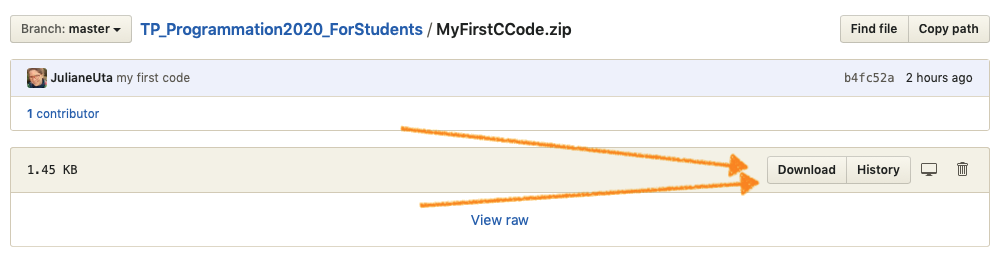
\includegraphics[width=0.6\textwidth]{Plots/FirstCode_1.png}
%\caption{Resultat de pacman -S mingw-w64-x86\_64-pkg-config mingw-w64-x86\_64-gtk3 make}
\end{figure}
Le dossier se trouvera dans votre dossier de téléchargements, voir ci-dessous.
\begin{figure}[H]
\center
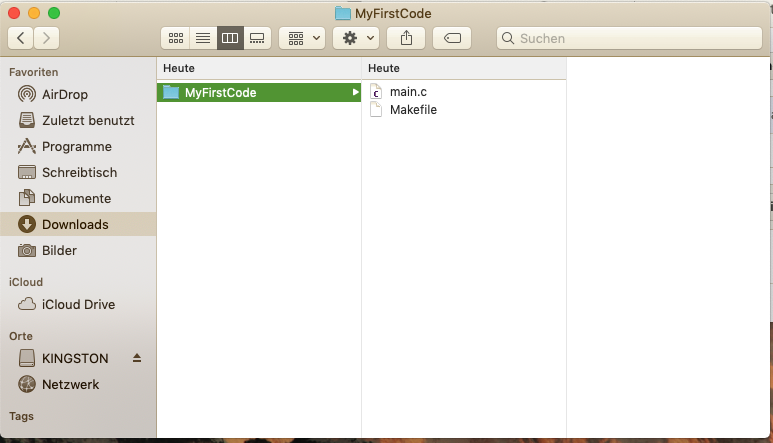
\includegraphics[width=0.6\textwidth]{Plots/DownloadMyFirstCode.png}
\caption{Le dossier Downloads dans le finder.\label{F:locationMyFirstCode}}
\end{figure}
Cliquez sur main.c pour l'ouvrir. 

Si le fichier ne s'ouvre pas avec l'éditeur de code que vous avez installé sur votre ordinateur (par exemple : Xcode, ou Atom, ou Visual Studio Codes), faites un clic droit sur main.c, puis sélectionnez Information. 

La fenêtre suivante devrait s'ouvrir. Vous devez naviguer jusqu'à « ouvrir avec » et sélectionner votre éditeur de code. Vous devez ensuite cliquer sur « modifier/changer tout  » pour appliquer ce choix à tous les fichiers qui se terminent par « .c ».
\begin{figure}[H]
\begin{subfigure}[c]{0.5\textwidth}
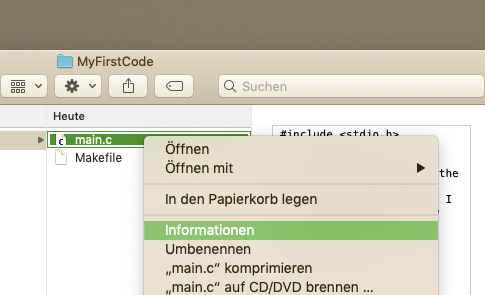
\includegraphics[width=0.95\textwidth]{Plots/OpenMain.png}
\subcaption{clic droit sur main.c, puis sélectionnez Information}
\end{subfigure}
\begin{subfigure}[c]{0.5\textwidth}
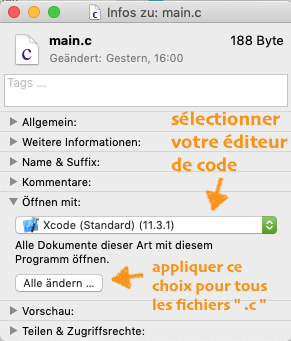
\includegraphics[width=0.75\textwidth]{Plots/OpenMain2.png}
\subcaption{sélectionner votre éditeur de code et cliquer sur « modifier/changer tout  »}
\end{subfigure}
\caption{Si main.c ne s'ouvre pas avec l'éditeur de code.}
\end{figure}
Dans votre éditeur de code, le contenu de main.c devrait ressembler à ceci.
\begin{figure}[H]
\center
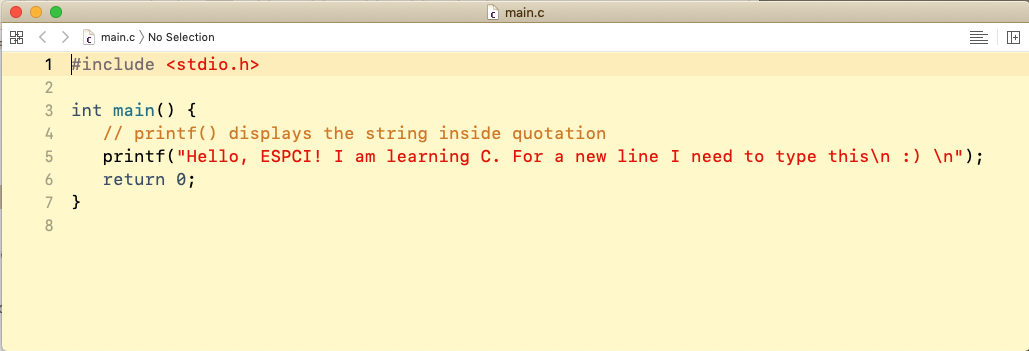
\includegraphics[width=0.6\textwidth]{Plots/ContentMain.png}
%\caption{Resultat de pacman -S mingw-w64-x86\_64-pkg-config mingw-w64-x86\_64-gtk3 make}
\end{figure}
Nous voulons maintenant compiler le code (traduire ces mots écrits en quelque chose qui puisse être interprété par l'ordinateur). {\color{Bittersweet}\textbf{Soyez attentifs, car c'est ce que vous ferez de manière extensive pendant ce TP.}}

Vous devez lancer l'application appelée Terminal (voir \fig{F:HowToFindTerminal}).

Votre terminal se trouve toujours dans un répertoire quelconque. Si vous tapez 
\begin{tcolorbox}[width=\textwidth,colframe=Bittersweet,colback={black},title={Ceci est le terminal},outer arc=0mm,colupper=white]    
      \large\textbf{pwd}
\end{tcolorbox}
et confirmez avec ENTER, vous verrez dans quel dossier se trouve actuellement le terminal. 
\begin{figure}[H]
\center
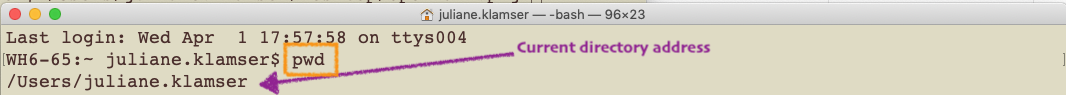
\includegraphics[width=1\textwidth]{Plots/Pwd.png}
%\caption{Resultat de pacman -S mingw-w64-x86\_64-pkg-config mingw-w64-x86\_64-gtk3 make}
\end{figure}
Si vous utilisez la commande (ls comme « \textbf{l}i\textbf{s}t everything that is here »)
\begin{tcolorbox}[width=\textwidth,colframe=Bittersweet,colback={black},title={Ceci est le terminal},outer arc=0mm,colupper=white]    
      \large\textbf{ls}
\end{tcolorbox}
dans votre terminal et que vous confirmez avec ENTREE, vous verrez une \textbf{l}i\textbf{s}te de tous les dossiers et documents qui se trouvent dans le dossier actuel.
\begin{figure}[H]
\center
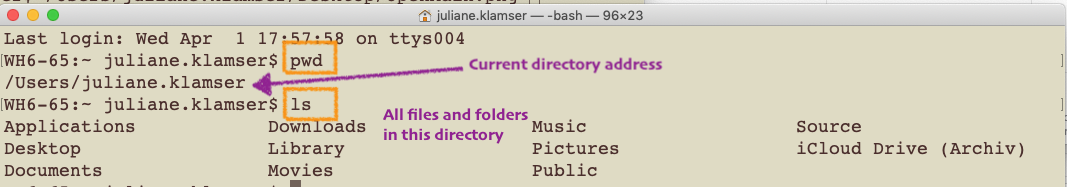
\includegraphics[width=1\textwidth]{Plots/LS.png}
%\caption{Resultat de pacman -S mingw-w64-x86\_64-pkg-config mingw-w64-x86\_64-gtk3 make}
\end{figure}
{\color{Bittersweet}\textbf{Attention :}} Peut-être votre finder vous montrera-t-il tout en français (vous voyez sur l'image que la langue du finder est l'allemand dans ce cas). Toutefois, il ne s'agit que d'un \textbf{maquillage}. Ce n'est pas la véritable langue de votre ordinateur. Si vous utilisez la commande ls, vous verrez que tous les dossiers ont des noms \textbf{ANGLAIS} et dans le terminal vous devez travailler avec les noms \textbf{ANGLAIS}.

Pour compiler et exécuter le code main.c, nous devons d'abord naviguer dans le terminal jusqu'au dossier où se trouve le code. Vous pouvez changer de dossier avec la commande (Attention, ce qui suit n'est qu'une syntaxe avec un chemin absurde. N'exécutez pas la commande suivante !)
\begin{tcolorbox}[width=\textwidth,colframe=Bittersweet,colback={black},title={Ceci est le terminal},outer arc=0mm,colupper=white]    
      \large\textbf{cd Path/Of/Directory/}
\end{tcolorbox}

Supposons que vous n'ayez pas déplacé le code après le téléchargement et que le dossier MyFistCode se trouve toujours dans le dossier Downloads (voir \fig{F:locationMyFirstCode}). Dans ce cas, suivez les étapes suivantes pour naviguer sur le terminal dans le dossier MyFirstCode.
Tapez la commande suivante pour vous rendre au répertoire d'origine et confirmez avec ENTER
\begin{tcolorbox}[width=\textwidth,colframe=Bittersweet,colback={black},title={Ceci est le terminal},outer arc=0mm,colupper=white]    
      \large\textbf{cd}
\end{tcolorbox}
Tapez la commande suivante et confirmez avec ENTER pour vous rendre dans le dossier MyFirstCode
\begin{tcolorbox}[width=\textwidth,colframe=Bittersweet,colback={black},title={Ceci est le terminal},outer arc=0mm,colupper=white]    
      \large\textbf{ cd Downloads/MyFirstCode/}
\end{tcolorbox}
Si vous utilisez maintenant la commande 
\begin{tcolorbox}[width=\textwidth,colframe=Bittersweet,colback={black},title={Ceci est le terminal},outer arc=0mm,colupper=white]    
      \large\textbf{ ls}
\end{tcolorbox}
vous devriez obtenir la sortie suivante (il y a deux fichiers : Makefile et main.c)
\begin{figure}[H]
\center
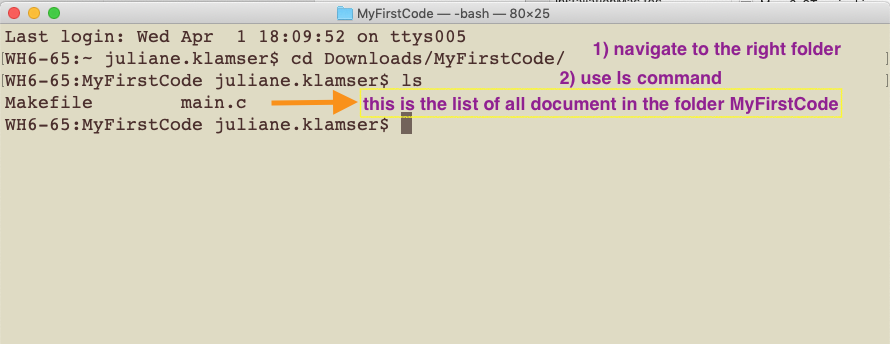
\includegraphics[width=1\textwidth]{Plots/navigateToMyFirstCode.png}
%\caption{Resultat de pacman -S mingw-w64-x86\_64-pkg-config mingw-w64-x86\_64-gtk3 make}
\end{figure}
Pour compiler le code, que vous avez vu dans votre éditeur du code, tapez
\begin{tcolorbox}[width=\textwidth,colframe=Bittersweet,colback={black},title={Ceci est le terminal},outer arc=0mm,colupper=white]   
      \large\textbf{ make}
\end{tcolorbox}
Vous devriez voir une sortie comme celle-ci.
\begin{figure}[H]
\center
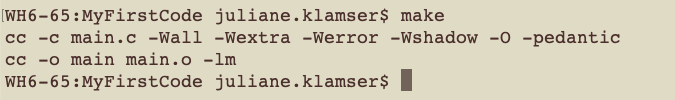
\includegraphics[width=0.9\textwidth]{Plots/FirstCode_6.png}
\end{figure}
Si vous tapez maintenant 
\begin{tcolorbox}[width=\textwidth,colframe=Bittersweet,colback={black},title={Ceci est le terminal},outer arc=0mm,colupper=white]   
      \large\textbf{ ls}
\end{tcolorbox}
Vous devriez voir une sortie comme celle-ci. Il existe deux autres fichiers, main.o et main (sans « .o » ou « .c »). main est écrit dans une langue que l'ordinateur peut interpréter et exécuter. C'est ce que l'on appelle l'exécutable.
 \begin{figure}[H]
\center
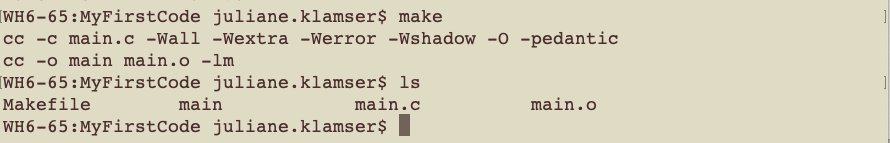
\includegraphics[width=0.9\textwidth]{Plots/FirstCode_7.png}
\end{figure}
Pour exécuter le main, tapez
\begin{tcolorbox}[width=\textwidth,colframe=Bittersweet,colback={black},title={Ceci est le terminal},outer arc=0mm,colupper=white]   
      \large\textbf{ ./main}
\end{tcolorbox}
Vous devriez voir une sortie comme celle-ci. 
\begin{figure}[H]
\center
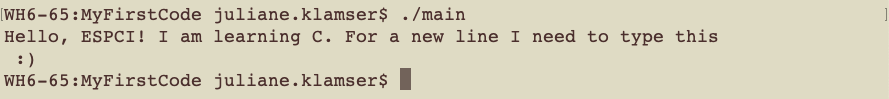
\includegraphics[width=0.9\textwidth]{Plots/FirstCode_8.png}
\end{figure}
Il s'agit de la sortie du code. Si vous voyez ce résultat, alors félicitations à vous. Vous êtes maintenant prêt à commencer le TP.

\section{Test pour le projet final}
Nous devons tester si votre ordinateur est prêt pour le projet final.

Allez à la page suivante et cliquez sur "Download" : \\ \href{https://github.com/JulianeUta/TP_Programmation2020_ForStudents/blob/master/MDFlexBoxRadiusMass.zip}{https://github.com/JulianeUta/TP\_Programmation2020\_ForStudents/blob/master/MDFlexBoxRadiusMass.zip}.

Extrayez le dossier « MDFlexBoxRadiusMass » (clic droit sur le dossier $\rightarrow$ extraire tout). 

Naviguez le terminal à l'intérieur du dossier « MDFlexBoxRadiusMass ». Notez que si vous avez déjà utilisé cd /path/to/folder/, vous n'êtes peut-être pas dans le répertoire d'origine. Avec la commande pwd, vous pouvez voir dans quel dossier se trouve le terminal en ce moment.
\begin{tcolorbox}[width=\textwidth,colframe=Bittersweet,colback={black},title={Ceci est le terminal},outer arc=0mm,colupper=white]  
    \large\textbf{  pwd }
\end{tcolorbox}
Vous devrez peut-être d'abord naviguer vers le dossier d'origine avec la commande
\begin{tcolorbox}[width=\textwidth,colframe=Bittersweet,colback={black},title={Ceci est le terminal},outer arc=0mm,colupper=white]  
    \large\textbf{  cd }
\end{tcolorbox}
ou vous pouvez aussi revenir en arrière sur une couche du dossier avec la commande
\begin{tcolorbox}[width=\textwidth,colframe=Bittersweet,colback={black},title={Ceci est le terminal},outer arc=0mm,colupper=white]  
    \large\textbf{  cd ..}
\end{tcolorbox}
et ensuite naviguer de là vers l'intérieur du dossier « MDFlexBoxRadiusMass ».

Une fois que vous êtes dans le bon dossier ( « MDFlexBoxRadiusMass »), tapez
\begin{tcolorbox}[width=\textwidth,colframe=Bittersweet,colback={black},title={Ceci est le terminal},outer arc=0mm,colupper=white]  
    \large\textbf{  ls }
\end{tcolorbox}
Votre résultat devrait ressembler à ceci
\begin{figure}[H]
\center
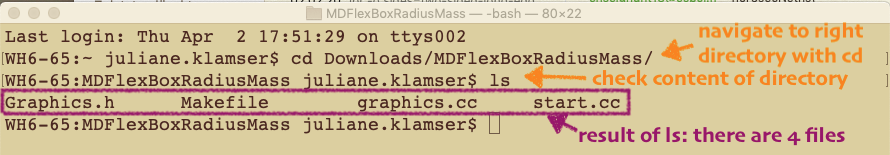
\includegraphics[width=0.9\textwidth]{Plots/MD_2CD.png}
\end{figure}
Maintenant, compilez le code avec
\begin{tcolorbox}[width=\textwidth,colframe=Bittersweet,colback={black},title={Ceci est le terminal},outer arc=0mm,colupper=white]  
    \large\textbf{  make }
\end{tcolorbox}
et listez à nouveau tous les fichiers avec
\begin{tcolorbox}[width=\textwidth,colframe=Bittersweet,colback={black},title={Ceci est le terminal},outer arc=0mm,colupper=white]  
    \large\textbf{  ls }
\end{tcolorbox}
Vous devriez voir trois nouveaux fichiers (graphics.o, start.o et start) comme ici
\begin{figure}[H]
\center
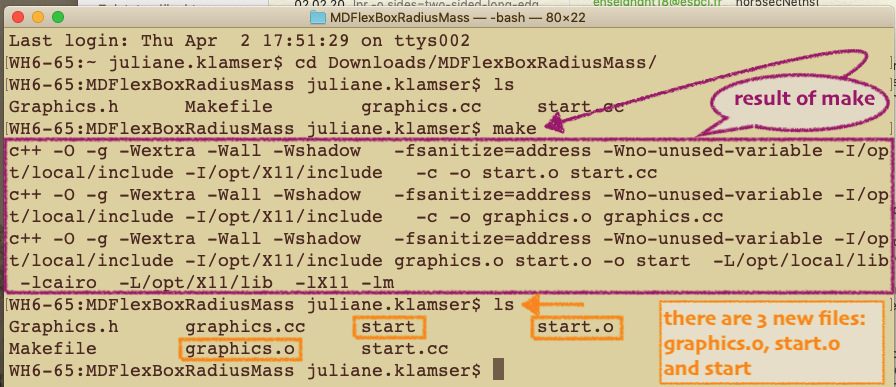
\includegraphics[width=0.9\textwidth]{Plots/MD_3Make.png}
\end{figure}
Dans ce cas, l'exécutable est appelé start. Nous lançons l'exécutable avec la commande suivante
\begin{tcolorbox}[width=\textwidth,colframe=Bittersweet,colback={black},title={Ceci est le terminal},outer arc=0mm,colupper=white]  
    \large\textbf{  ./start }
\end{tcolorbox}
Une fenêtre XQuartz devrait s'ouvrir comme ici
\begin{figure}[H]
\center
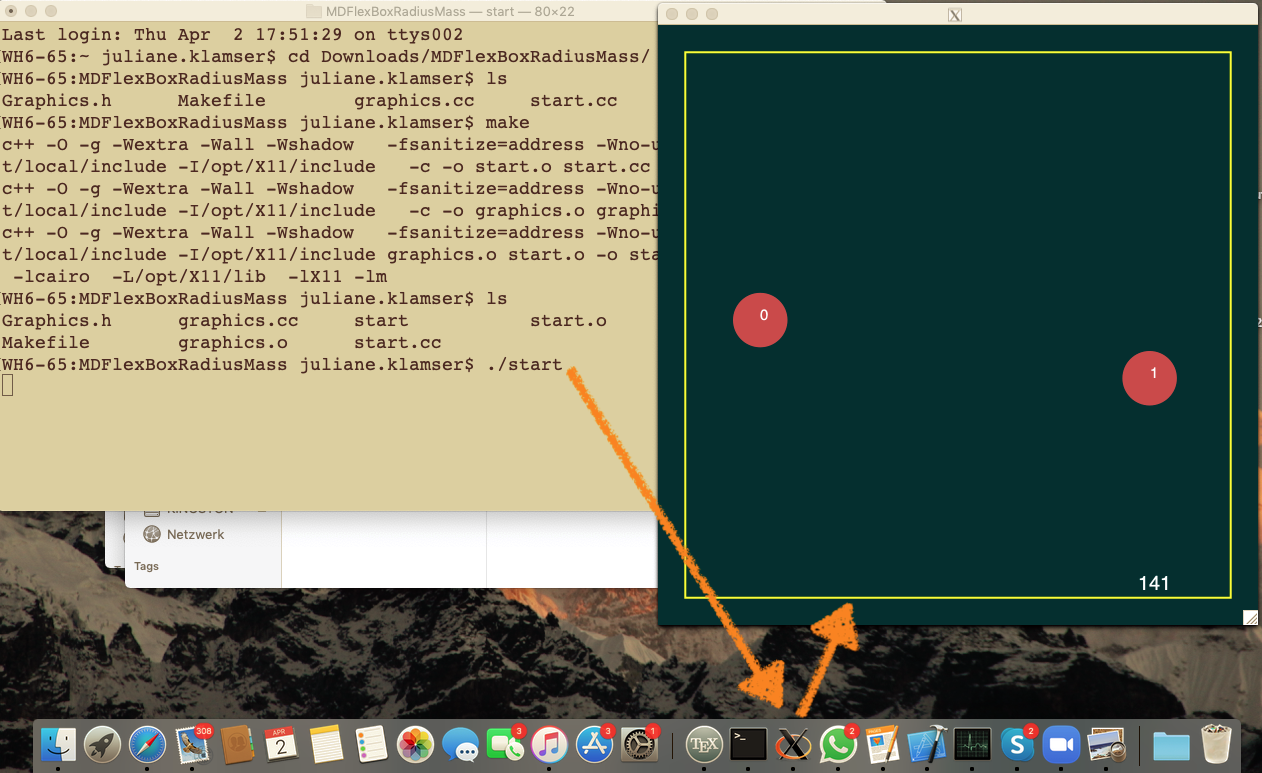
\includegraphics[width=0.9\textwidth]{Plots/MD_4XQuartz.png}
\end{figure}
Vous devriez voir un carré vert avec deux particules rouges à l'intérieur et un petit compteur blanc en bas à droite qui augmente.
\subsection{Troubleshooting}
Si vous ne voyez pas la fenêtre XQuartz avec les cercles rouges?

Recherchez l'application XQuartz, que vous avez installée dans le chapitre \ref{S:InstallXquatz}. Vous pouvez effectuer une recherche avec Spotlight ou vous rendre dans le même dossier, où vous avez trouvé l'application Terminal /Applications/Utilities/ (voir \fig{F:HowToFindTerminal}). 

Ouvrez l'application XQuartz. XQuartz dispose de son propre terminal. Nous voulons ouvrir ce terminal maintenant et y lancer le code. Pour ouvrir le terminal XQuartz, suivez les indications de l'image ci-dessous.
\begin{figure}[H]
\center
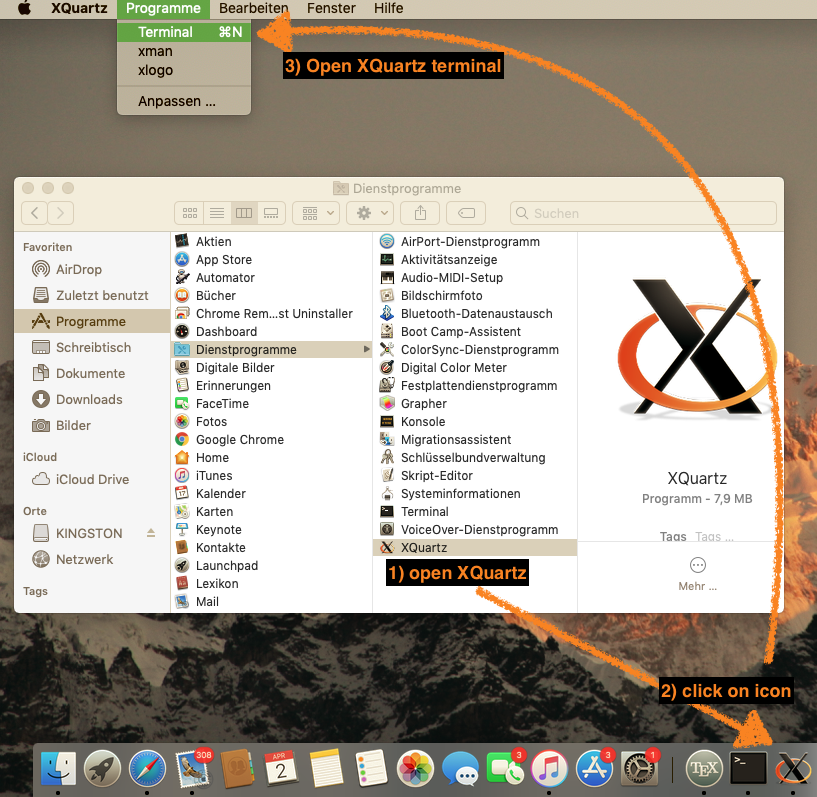
\includegraphics[width=0.9\textwidth]{Plots/TroubleshootingMD.png}
\end{figure}
Vous devriez voir quelque chose comme dans l'image ci-dessous. Ce terminal fonctionne de la même manière que l'autre terminal.
\begin{figure}[H]
\center
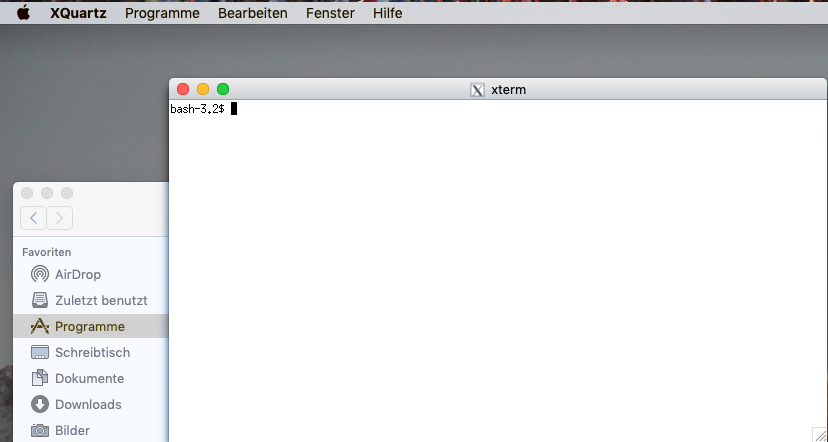
\includegraphics[width=0.75\textwidth]{Plots/XQuartzTerminal.png}
\end{figure}
Encore une fois, vous devez naviguer sur ce terminal à l'intérieur du dossier « MDFlexBoxRadiusMass ». Ensuite, exécutez le code avec
\begin{tcolorbox}[width=\textwidth,colframe=Bittersweet,colback={black},title={Ceci est le terminal},outer arc=0mm,colupper=white]  
    \large\textbf{  ./start }
\end{tcolorbox}
Vous devriez voir cela maintenant
\begin{figure}[H]
\center
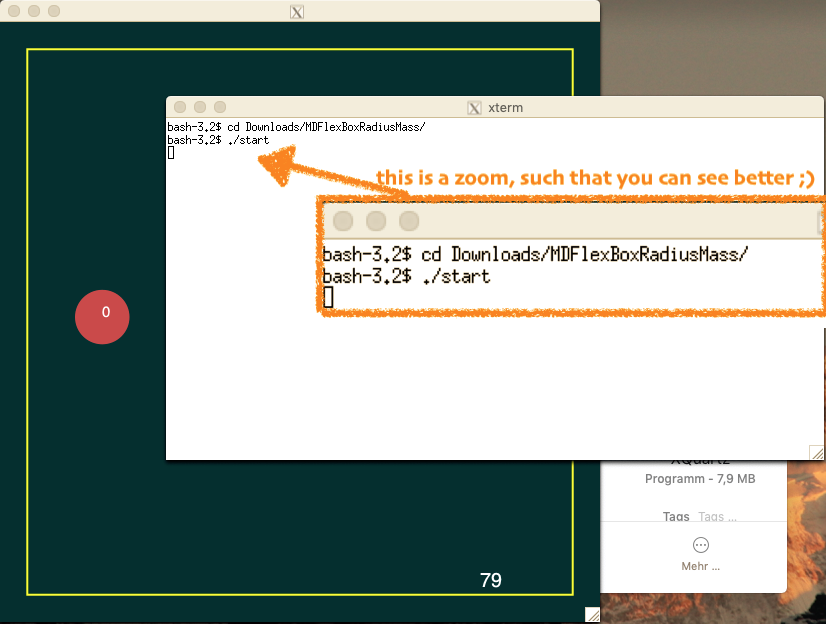
\includegraphics[width=0.75\textwidth]{Plots/XQuartzFinal.png}
\end{figure}

Si vous ne voyez pas la fenêtre XQuartz avec les cercles rouges?, contactez \href{mailto:example@example.com}{juliane.klamser@espci.psl.eu}.

\subsection{Comment travailler simultanément avec quelqu'un d'autre sur le même code ?}
Comme mentionné au chapitre \ref{S:VisCodAtom}, vous pouvez utiliser les fonctions intégrées des éditeurs de code Visual Studio Code ou Atom. 

Une autre méthode professionnelle, qu'il convient de mentionner, est GitHub. Elle est très puissante et largement utilisée. Cependant, elle nécessite une certaine formation.

La méthode la plus simple est de créer un compte dropbox et d'utiliser dropbox paper. Si vous copiez votre code dans le fichier du dropbox paper, vous et votre partenaire pouvez travailler sur le même code en même temps.
%\bibliographystyle{unsrt}  
%\bibliography{references}  %%% Remove comment to use the external .bib file (using bibtex).
%%% and comment out the ``thebibliography'' section.

\end{document}
